The jumping and landing example was designed to introduce the \emph{bioptim}'s ability to reduce the number of degrees-of-freedom (DoF) of a model, to include nonlinear boundaries on controls, and to solve complex multiphase programs that include impacts.
The main goal of the jumper is (without much of a surprise) to jump as high as possible.

The full body model consists of 3 DoF at the pelvis (the forward and upward translation, and the tranverse rotation), 2 DoF at each upper limb (shoulder flexion and abduction), and 3 DoF at each lower limb (hip, knee and ankle flexion) for a total of 13 DoF.
For this optimization, the shoulder abduction of both sides DoF are ignored and the model is symmetrized by using \emph{BidirectionalMapping}, effectively creating a 7 DoF pseudo-2D model. 
Since this is a full body model, the root segment (i.e., the pelvis) is uncontrolled, reducing the number of control variables to 4, namely the shoulder, hip, knee and ankle flexion. 


The goal was to find a minimal-time push-off phase for a \hl{XXX-DoF torque-driven} model while maximizing its jump height ($h$).
The push-off (impulsion before take-off) was divided into two phases with the following properties: \emph{1)} two contact points (heel and toe), duration $\in [0.2, 1.0]s$ and \emph{2)} one contact (toe), duration $\in [0.05, 1.0]s$.
The joint actuators bounds were modeled using a custom nonlinear constraint to account for torque/angle/angular-velocity relationships using the \verb?gauss3p? function of \emph{biorbd} \comment{based on predetermined factors}{je ne comprends pas} (\ref{fig:graph_force_vitesse_longueur}).
For each phase, the objective function was formulated as follow:

\[
\mathcal{J} = XXX.
\addtag
\label{eq:cost_jumper}
\]

The first term of Eq.~\ref{eq:cost_jumper} corresponds to maximizing the jump height.
The second term of the objective function serves for finding a minimal-time solution.

Using \emph{ipopt}, the problem was first approximately solved using the BFGS hessian approximation for 200 iterations maximum.
Then, \comment{if this maximum number of iterations was reached}{ne parler que de la solution présentée. Est-ce que le max_iter a effectivement été atteint ?}, the solution was re-optimized, using a warm-start, with exact-hessian computations for up to 1000 iterations .

The optimized ump height was 1,35m in \hl{XXX}s.
\comment{The used strategy is XXX with a proximo-distal shift of the joints (hip, knee then ankle) highlighted by the activation of the hip, then the knee and finally the ankle.}{à terminer}

\begin{figure}[h!]
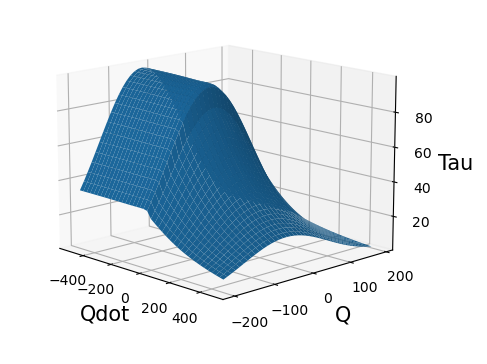
\includegraphics[width=\columnwidth]{../figures/graph_force_vitesse_longueur.png}\\
\caption{Surface representing the nonlinear constraint which account for torque/angle/angular-velocity relationships in the model of the jumper.}
\label{fig:graph_force_vitesse_longueur}
\end{figure}
